
\subsection{General Equation of Motion}
The state of the electron hydrogen
system at a given time can be completely
characterised by its density
matrix.
Working in the interaction
picture, a general density matrix
\(\hat{\rho}(t)\) time evolves according
to the von Neumann equation~\cite{TP2_Notes}.
\begin{equation}
    \frac{d\hat{\rho}_t(t)}{dt} =
    -i [\hat{H}_{int}(t), \hat{\rho}_t(t)]
    \label{eqn:density equation of motion}
\end{equation}
which can be integrated to give
\begin{equation}
    \hat{\rho}_t(t) =
    \hat{\rho}_t(0)
    - i \int_0^t ds
        [\hat{H}_{int}(s), \hat{\rho}_t(s)]
    \label{eqn:integrated density equation of motion}
\end{equation}
We can expand this equation of motion
to second order in the interaction
by substituting \cref{eqn:integrated density equation of motion}
into \cref{eqn:density equation of motion}
twice to give
\begin{equation}
    \frac{d\hat{\rho}_t(t)}{dt} =
    -i [\hat{H}_{int}(t), \hat{\rho}_t(0)]
    - \int_0^t ds
        [\hat{H}_{int}(s),
            [\hat{H}_{int}(s), \hat{\rho}_t(t)]]
    +\mathcal{O}({\hat{H}_{int}}^3)
\end{equation}
It is possible to reduce this to
an equation of motion
describing just the system by taking
a trace over the environment~\cite{Manzano_2020}
\begin{equation}
    \hat{\rho}(t) =
    -i Tr_e[\hat{H}_{int}(t), \hat{\rho}_t(0)]
    - \int_0^t ds
    Tr_e[\hat{H}_{int}(s),
    [\hat{H}_{int}(s), \hat{\rho}_t(t)]]
    \label{eqn:density motion before redfield approximation}
\end{equation}
where \(\hat{\rho}(t) = Tr_e[\hat{\rho}_t(t)]\)
is the density operator of the system.
Using a clever re-definition of the interaction
Hamiltonian~\cite{Manzano_2020} it
is possible to show that the first
term gives no contribution to the
overall dynamics of the system.

\subsection{The Redfield Assumption}\label{sec:the redfield assumption}
To arrive at the Redfield equation
we first make the assumption that the
system and surrounding density
matrix is completely
decoupled~\cite{theory_open_quantum_systems},
allowing us to write
\begin{equation}
    \hat{\rho}_t(t) = \hat{\rho}(t) \otimes \hat{\rho}_E(t)
\end{equation}
where \(\hat{\rho}_E(t)\), the
density matrix of the environment,
is taken as a purely statistical ensemble.
Under the Markov approximation
we can extend the upper limit
of \cref{eqn:density motion before redfield approximation}
to \(\infty \), arriving at the Redfield
equation
\begin{equation}
    \dot{\hat{\rho}}(t) =
    - \int_0^{\infty} ds
    Tr_{E}[\hat{H}_{int}(t),
            [\hat{H}_{int}(s-t),
                    \hat{\rho}(t) \otimes \hat{\rho}_E(t)]]
\end{equation}
Separating out the interaction hamiltonian
into system and surroundings according
to~\cref{eqn:split interaction hamiltonian}
\begin{align}
    \hat{H}_{int} & = \sum_{i,j} \hat{S}_{i,j} \hat{E}_{i,j}
\end{align}
we can simplify the form of this equation to give~\cite{Manzano_2020}
\begin{equation}
    \dot{\hat{\rho{}}}(t) = \begin{aligned}[t]
        \sum_{i,j,k, l} &
        \exp{(-i(\omega_{i,j}-\omega_{k,l})t)}
        \Gamma_{i,j;k, l}(\omega_{k,l})
        [S_{k, l}\hat{\rho}(t),
        S^\dagger_{i,j}]  \\
        +               &
        \exp{(i(\omega_{i,j}-\omega_{k,l}))}
        \Gamma^*_{k, l; i,j}(\omega_{i,j})
        [S_{k, l},
            \hat{\rho}(t) S^\dagger_{i,j}]
    \end{aligned} \label{eqn:redfield equation gamma form}
\end{equation}
where \(\Gamma \) is given by
\begin{equation}
    \Gamma_{i,j, k,l}(\omega) =
    \int_0^\infty{}{
    ds \exp{(i\omega{}s)}
    Tr_{E}[E^\dagger_{i,j}(t)E_{k,l}(t-s)\rho_E(0)]
    }\label{eqn:gamma definition}
\end{equation}

\subsection{The Lindblad Equation}
To obtain the Lindblad equation
we need to apply the rotating
wave approximation to
\cref{eqn:redfield equation gamma form}.
Before applying this
we first expand out the commutators
in \cref{eqn:redfield equation gamma form}
\begin{align}
    \bra{m}[S_{k, l}\hat{\rho}(t),
    S^\dagger_{i, j}] \ket{n}              & =
    \sum_{\alpha, \beta} \rho_{\alpha, \beta} [
        \delta_{m, k}\delta_{l, \alpha}
        \delta_{\beta, j}\delta_{i, n}
        -\delta_{m, j}\delta_{i, k}
    \delta_{l, \alpha}\delta_{\beta, n}]       \\
    \bra{m}[S_{k, l},
    \hat{\rho}(t)S^\dagger_{i, j}] \ket{n} & =
    \sum_{\alpha, \beta} \rho_{\alpha, \beta} [
        \delta_{m, k}\delta_{l, \alpha}
        \delta_{\beta, j}\delta_{i, n}
        -\delta_{m, \alpha}\delta_{\beta, j}
        \delta_{i, k}\delta_{l, n}]
\end{align}
which we use to obtain an expanded
form of \(\gamma{}\)
\begin{equation}
    \bra{m}\dot{\hat{\rho}}(t) \ket{n} = \begin{aligned}[t]
        \sum_{i,j,k, l, \alpha, \beta} &
        \exp{(-i\Delta{}Et)}
        \Gamma_{i,j;k, l}(\omega_{k,l})
        \rho_{\alpha, \beta} [         &
            \delta_{m, k}\delta_{l, \alpha}
        \delta_{\beta, j}\delta_{i, n}                          \\
                                       &                      &
            -\delta_{m, j}\delta_{i, k}
        \delta_{l, \alpha}\delta_{\beta, n}]                    \\
        +                              & \exp{(i\Delta{}E t)}
        \Gamma^*_{k, l; i,j}(\omega_{i,j})
        \rho_{\alpha, \beta} [         &
            \delta_{m, k}\delta_{l, \alpha}
        \delta_{\beta, j}\delta_{i, n}                          \\
                                       &                      &
            - \delta_{m, \alpha}\delta_{\beta, j}
            \delta_{i, k}\delta_{l, n}]
    \end{aligned}
\end{equation}
the rotating wave approximation
limits us to two cases
\begin{itemize}
    \item \(i=j\), \(k=l\)
    \item \(i=k\), \(j=l\)
\end{itemize}
Imposing this condition using the expression
\(\delta_{i,j}\delta_{k,l}
+ \delta_{i,k}\delta_{j,l}
- \delta_{i,j}\delta_{k,l}
\delta_{i,k}\)
we come to the lindblad
equation
\begin{equation}
    \bra{m}\dot{\hat{\rho}}(t) \ket{m}  = \begin{aligned}[t]
        [ & 2\Gamma_{m,\neq m;m, \neq m}(\omega_{m,\neq m})\rho_{\neq m, \neq m} \\
        - & 2\Gamma_{\neq m,m;\neq m, m}(\omega_{\neq m,m})\rho_{m, m}]
    \end{aligned}
\end{equation}
where the off diagonal
terms vanish assuming the
density matrix is initially
purely diagonal. A full derivation
of this expression can be found in
\cref{app:redfield to lindblad}.



\subsection{Calculating \(\Gamma \)}
Using \cref{eqn:gamma definition}
we can calculate the value of \(\Gamma \).
The
density matrix of a purely
statistical ensemble is given
by~\cite{sakurai_napolitano_2020}
\begin{equation}
    \rho_E(0) = \sum_{\{N(k)\}}
    P(\{N(k)\})
    \ket{N(k)} \bra{N(k)}
\end{equation}
and
\begin{equation}
    \hat{E}_{i,j} = \sum_{k,s,k',s'}
    {\tilde{V}_{eff}(\vec{q})}_{i,j}
    \hat{b}^\dagger_{k',s'}\hat{b}_{k,s}
\end{equation}
where we assume the potential
is independent of \(q\). We can
take the trace over the
environment (todo reference)
\begin{equation}
    Tr_E[\dots]  = \begin{aligned}[t]
        \sum_{\substack{\{N(k)\}                             \\
        k_1,s^1,k_2,s^2                                      \\
                k_3,s^3,k_4,s^4 }}
         & P(\{N(k)\}) V_{i,j} V_{k,l}                       \\
         & \exp{(i(E_1 - E_2) t)} \exp{(i(E_3 - E_4) (t-s))} \\
         & \bra{N(k)}
        \hat{b}_{k_1,s^1}^\dagger{} \hat{b}_{k_2,s^2}
        \hat{b}_{k_3,s^3}^\dagger{} \hat{b}_{k_4,s^4}
        \ket{N(k)}
    \end{aligned}
\end{equation}
where \( \{N(k)\} \) is the set of
all possible occupations, and
the boltzmann
probability associated with a
given state is
\(P(\{N(k)\}) = \exp{(-\beta{}(E-\mu N))}\).
The trace is only non zero in two
cases
\begin{itemize}
    \item \(k_1=k_2, s^1=s^2\),
          \(k_3=k_4, s^3=s^4\)
    \item \(k_1=k_4, s^1=s^4\),
          \(k_3=k_2, s^3=s^2\) but
          \(k_1\neq{}k_2, s^1\neq{}s^2\)
\end{itemize}
and we can therefore obtain the
simplified form of the trace (reference)
\begin{equation}
    Tr_E[\dots] = \begin{aligned}[t]
        \sum_{k_1,s^1,k_3,s^3 }
         & V_{i,j} V_{k,l} [ \\
         & N_1 N_3
                + N_1 (1 - N_3) \exp{(-i(E_3 - E_1)s)}]
    \end{aligned}
\end{equation}
Integrating over \(s\) we obtain
an additional constant on the
wavevectors, and after
converting the sum into
an integral and re-adsorbing
the power of \(L^3\) into the
definition of (reference)
\begin{align}
    \Gamma_{i,j, k,l}(\omega) & =\begin{aligned}[t]
        \sum_{s^1,s^3} \int &
        \frac{d^3\vec{k}_1}{{(2\pi)}^3}
        \frac{d^3\vec{k}_3}{{(2\pi)}^3}
        V_{i,j} V_{k,l} [
        N_1 N_3 \delta_{w, 0} \frac{m}{\sqrt{k_3^2}} \\
                            & + N_1 (1 - N_3)
                \frac{m}{\sqrt{k_1^2 - 2m\omega}}
                \delta({k_3 \pm \sqrt{k_1^2 + 2m\omega}}) ]
    \end{aligned}
\end{align}
The first term is divergent (reference)
but we find no terms in the \ldots
with \(\omega = 0\).
We evaluate the second term
by expanding about the fermi
wavevector
\begin{equation}
    \Gamma_{i,j, k,l}(\omega_{k,l}) =\begin{aligned}[t]
        \sum_{s^1,s^3} \exp{(\frac{\beta \omega_{k,l}}{2})} \frac{m k_f^2 }{{(2\pi)}^4}
        V_{i,j} V_{k,l} \sqrt{\pi} \frac{2m}{\beta \hbar^2}
    \end{aligned}
\end{equation}
substituting in the expression
for v (reference)
we arrive at the final
expression for \(\Gamma \)
\begin{equation}
    \sum_{s^1,s^3} \exp{(\frac{\beta \omega_{k,l}}{2})}
    \mathcal{C}_{i,j} \mathcal{C}_{k,l}
    \sqrt{\pi} \frac{8 k_f^2 \epsilon_0^2 \hbar^3}{\beta e^4 m^2}
\end{equation}

\subsection{}
we arrive at the final form of
the Lindblad equation
for our system
\begin{equation}
    \bra{m}\dot{\hat{\rho{}(t)}} \ket{m} = \begin{aligned}[t]
        [ & 2\Gamma_{m,\neq m;m, \neq m}(\omega_{m,\neq m})\rho_{\neq m, \neq m} \\
        - & 2\Gamma_{\neq m,m;\neq m, m}(\omega_{\neq m,m})\rho_{m, m}]
    \end{aligned}
\end{equation}
where
\begin{equation}
    \Gamma_{i,j, k,l}(\omega_{k,l})   =
    \exp{(\frac{\beta \omega_{k,l}}{2})}
    \mathcal{C}_{i,j} \mathcal{C}_{k,l}
    \sqrt{\pi} \frac{32 k_f^2 \epsilon_0^2 \hbar^3}{\beta e^4 m^2}
\end{equation}

\subsection{Analytic Solution to the Rotating Wave Approximation}
Since the form of the rotating
wave approximation is a simple
rate equation with two variables
it is possible to solve it analytically
\cref{app:combined tunnelling rates}.
From the expression above we find the
forward and backward tunnelling rate as
\begin{align}
    \gamma_0 & = 2\Gamma_{1,0;0, 1}(\omega_{1,0})       \\
             & = A \exp{(\frac{\beta \omega_{0,1}}{2})}
    \mathcal{C}_{1,0} \mathcal{C}_{0,1}                 \\
    \gamma_1 & = 2\Gamma_{0,1;1, 0}(\omega_{0,1})       \\
             & = A \exp{(\frac{\beta \omega_{1,0}}{2})} \\
\end{align}
where
\(A =
\mathcal{C}_{1,0} \mathcal{C}_{0,1}
\sqrt{\pi}
\frac{64 k_f^2 \epsilon_0^2 \hbar^3}{\beta e^4 m^2}\).
This gives a combined rate of
\begin{equation}
    \gamma_0 + \gamma_1 = 2A\cosh{(\frac{\beta (E_1 - E_0)}{2})}
    \label{eqn:theoretical rate lindblad equation}
\end{equation}
for an energy difference of
\(3.04\pm0.16\times{}10^{-21} J\)
(\cref{eqn:hydrogen energy difference})
we find a tunnelling rate of
\(6.1\times{}10^{8}s^{-1}\),
corresponding to a
tunnelling time of
\(1.6\times{}10^{-9}s\) at
\(150K\).


\begin{figure}
    \centering
    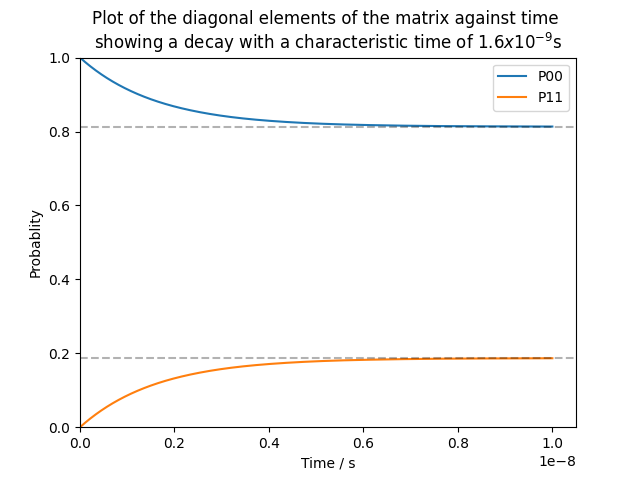
\includegraphics[width=.5\linewidth]{Figures/Redfield/Plot of lindblad solution.png}
    \caption{Plot of the Lindblad solution with a characteristic decay
    rate of \(6.1\times{}10^{8}s^{-1}\) at
    \(150K\).
    }\label{fig:two site lindblad soluton}
\end{figure}


\subsection{}
In reality there
are 3 HCP sites neighbouring
each FCC Hydrogen, all of which
are connected to 2 other HCP sites.
We should expect the tunnelling
rate to be at least
\(3\) times the single
neighbour rate TODO CITE MODEL CHAPTER s.
To investigate this behaviour we extend
the simulation to contain a large
grid of sites with periodic boundary conditions.
From this we find that the combined FCC occupation
falls at a rate of
\(1.8\times{}10^{9}s^{-1}\) at
\(150K\), exactly
three times the single neighbour rate (\cref{fig:multi site lindblad}).
\begin{figure}[htbp]
    \centering
    \begin{subfigure}{0.45\linewidth}
        \centering
        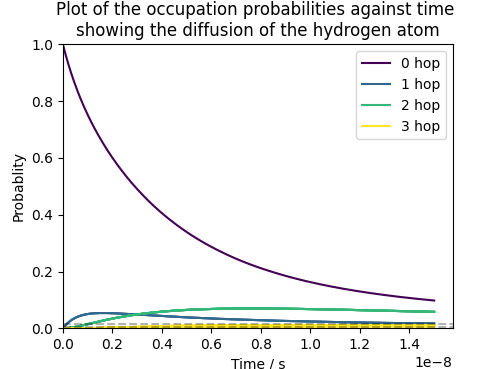
\includegraphics[width =0.9 \linewidth]{Figures/Redfield/Plot of lindblad solution many sites.png}
        \caption{Individual occupation probability
        }\label{sub@fig:multi site lindblad}
    \end{subfigure}
    \hfill
    \begin{subfigure}{0.45\linewidth}
        \centering
        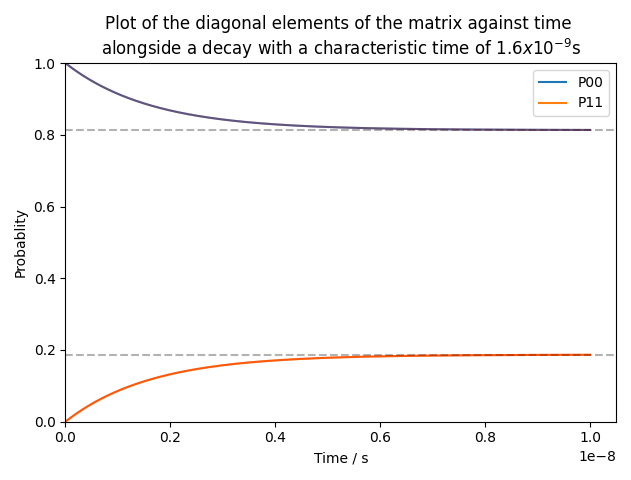
\includegraphics[width = 0.9\linewidth]{Figures/Redfield/Plot of redfield solution long time.png}
        \caption{Combined occupation probability
        }\label{sub@fig:multi site combined lindblad}
    \end{subfigure}
    \caption{Plot of the individual and combined
    occupation probabilities against time at
    \(150K\). The combined
    probability
    (\cref{sub@fig:multi site combined lindblad})
    follows exactly the same curve as in
    \cref{fig:two site lindblad soluton}
    with a rate of \(1.8\times{}10^{9}s^{-1}\).
    The plot of the individual occupation
    probabilities
    (\cref{sub@fig:multi site lindblad})
    shows that it takes
    a much longer time for the
    probability of occupation of the
    initial site to reach
    an equilibrium with the surroundings.}\label{fig:multi site lindblad}
\end{figure}
It is also possible to infer a
tunneling rate from the
individual probabilities.
Since these decay
exponentially we take the tunneling
time from the time taken for the
distance from equilibrium
to fall by \(\exp{(-1)}\).
For the initial
FCC site we can
take this equilibrium
to be the two site or
the three site occupation.
If we can also
use the time taken for the
neighbouring HCP sites to
reach their maximum occupation,
and half the time taken for the
neighbouring FCC to reach equilibrium.
The corresponding decay times are
given in \cref{tab:implied decay rates}.
\begin{table}[htbp]
    \begin{center}
        \begin{tabular}{ *{3}{c} }
            \toprule
            Measure                & Decay Time \(s\)                  & Implied Decay Rate \(s^{-1}\) \\
            \midrule
            Initial FCC            & \(4.54\times{}10^{-9}\)           & \(2.2\times{}10^{8}\)         \\
            Initial FCC (Two Site) & \(3.99\times{}10^{-10}\)          & \(2.5\times{}10^{9}\)         \\
            Next HCP               & \(4.37\times{}10^{-10}\)          & \(2.3\times{}10^{9}\)         \\
            Next FCC               & \(2\times{}1.31 \times{}10^{-9}\) & \(7.6\times{}10^{8}\)         \\
            Combined Occupation    & \(5.56\times{}10^{-10}\)          & \(1.8\times{}10^{9}\)         \\
            RMS Distance           & \(5.09\times{}10^{-10}\)          & \(2.0 \times 10^{9}\)         \\
            \bottomrule
        \end{tabular}
    \end{center}
    \caption{Implied decay rates
        from the probability
        distribution and RMS distance
        analysis at
        \(150K\).
        Since the individual
        probabilities undergo an exponential
        decay we take the decay time as
        the time for the probability to fall
        by \(\exp{(-1)}\).
        The RMS decay time corresponds
        to the time for the RMS distance
        to equal \(0.5\). Most measures
        of the decay rate take a similar
        amount of time, however the
        complete decay of the FCC
        occupation takes an order of
        magnitude longer.
    }\label{tab:implied decay rates}
\end{table}

\subsection{Distance Traveled}
We should also be able to
extract a tunneling time from
the root-mean squared (rms)
distance travelled by the
hydrogen. As the hydrogen
undergoes a random walk we should
expect the squared distance to
grow linearly with time.
\begin{figure}
    \centering
    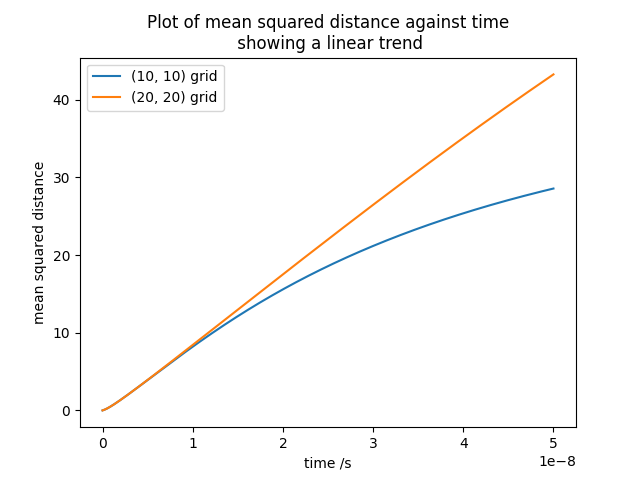
\includegraphics[width=0.5\linewidth]{Figures/Redfield/Plot of lindblad solution squared distance.png}
    \caption{Plot of the squared distance
    of the hydrogen atom against time
    showing a linear trend as expected
    for a random walk. The time taken
    for the rms distance to equal \(0.5\)
    is found to be
    \(5.09\times{}10^{-10}s\),
    which corresponds to an implied rate
    of \(2.0 \times 10^{9}s^{-1}\).
    }
\end{figure}
The tunneling time was
found to be \(5.25\times{}10^{-10}s\),
corresponding to teh time taken
for the rms distance to
reach \(0.5\). This gives
an overall rate of
\(1.9 \times 10^{9}s^{-1}\).

\subsection{Comparison with Experiment}
Given these measures of the
tunneling time it is now possible to compare
these tunneling rates to experiment.
In \cref{fig:tunneling rate against temperature}
the theoretical rates
are plotted against temperature
alongside the rates extracted
from the Lindblad analysis.
\begin{figure}[htbp]
    \centering
    \begin{subfigure}{0.45\linewidth}
        \centering
        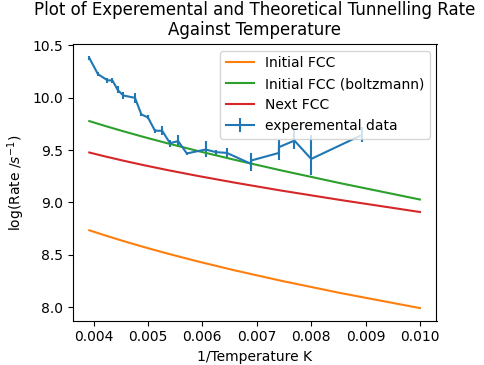
\includegraphics[width =0.9 \linewidth]{Figures/Redfield/Plot of redfield temperature dependance FCC points.png}
        \caption{FCC Tunneling Rates
        }\label{sub@fig:fcc tunneling rates temp dependence}
    \end{subfigure}
    \hfill
    \begin{subfigure}{0.45\linewidth}
        \centering
        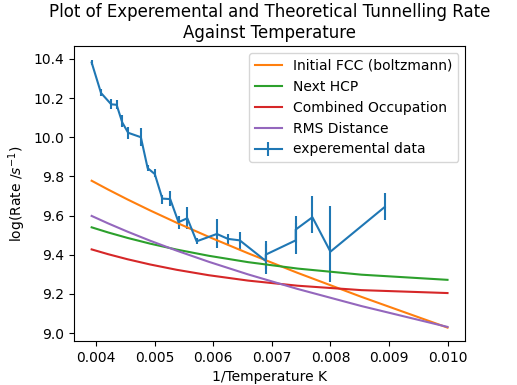
\includegraphics[width = 0.9\linewidth]{Figures/Redfield/Plot of redfield temperature dependance close points.png}
        \caption{Other Tunneling Rates
        }\label{sub@fig:other tunneling rates temp dependence}
    \end{subfigure}
    \caption{Plot of the tunneling
        rates against temperature, with comparison
        to the experimental data.
        The Initial and Next FCC tunneling rates
        (\cref{sub@fig:fcc tunneling rates temp dependence})
        deviate significantly from the experimental
        measurements, as well as many of the other
        measures of tunneling rate.
        The remaining rates however give
        a good fit to the experimental
        data
        (\cref{sub@fig:other tunneling rates temp dependence})
        although the temperature dependence
        is different for different measurements
        of the rate.
    }\label{fig:tunneling rate against temperature}
\end{figure}
Although the FCC tunneling
rates differ by an order of
magnitude the remaining
measurements of the rate
are similar to that measured
in experiment.
TODO-Temp dependance

\subsection{Assessing the Rotating Wave Approximation}
If we relax the rotating wave approximation
we arrive at the expression given in \cref{sec:redfield equation full solution}.
\begin{align}
    \bra{m}\dot{\hat{\rho{}}}(t) \ket{n} & = \begin{aligned}[t]
        \sum_{i,j} &
        \exp{(-i\Delta{}E_{n,j;m,i} t)}
        \Gamma_{n,j;m, i}(\omega_{m,i})
        \rho_{i,j}   \\
                   &
        -\exp{(-i\Delta{}E_{i,m;i,j} t)}
        \Gamma_{i,m;i, j}(\omega_{i,j})
        \rho_{j, n}  \\
                   &
        +\exp{(i\Delta{}E_{n,j;m,i} t)}
        \Gamma_{n,j; m, i}(\omega_{n,j})
        \rho_{i, j}  \\
                   &
        -\exp{(i\Delta{}E_{i,j;i,n} t)}
        \Gamma_{i,j; i, n}(\omega_{i,j})
        \rho_{m, j}
    \end{aligned}
\end{align}
This equation produces extra oscillations
on top of the Lindblad result, with
a characteristic timescales of
\(\frac{2\pi}{\omega_{1,0}} = 2.13\times{}10^{-13}s\). Plotting
the full solution (\cref{fig:redfield full solution})
however we see exactly the same behaviour as that
predicted by the lindblad result.
\begin{figure}[htbp]
    \centering
    \begin{subfigure}{0.45\linewidth}
        \centering
        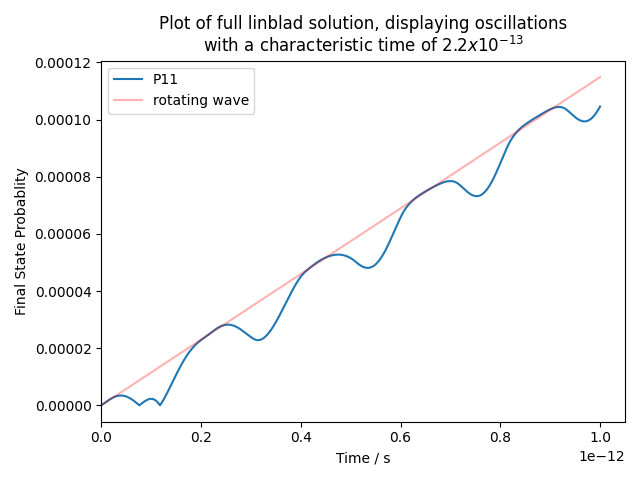
\includegraphics[width =0.9 \linewidth]{Figures/Redfield/Plot of redfield solution short time.png}
        \caption{Complete solution for small times
        }\label{fig:redfield full solution short timescales}
    \end{subfigure}
    \hfill
    \begin{subfigure}{0.45\linewidth}
        \centering
        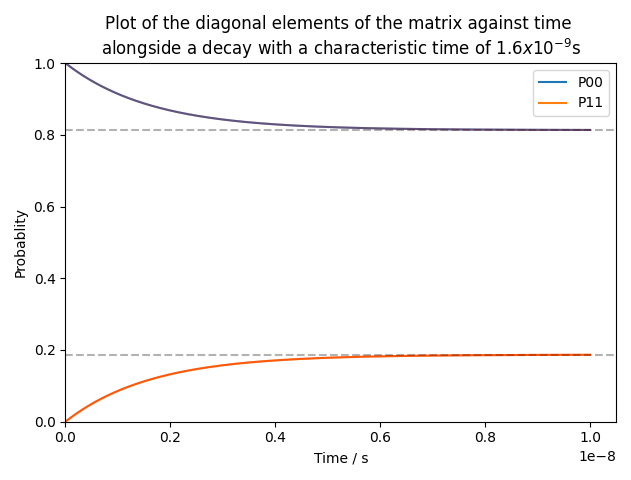
\includegraphics[width = 0.9\linewidth]{Figures/Redfield/Plot of redfield solution long time.png}
        \caption{Complete solution for long times
        }\label{fig:redfield full solution long timescales}
    \end{subfigure}
    \begin{subfigure}{0.45\linewidth}
        \centering
        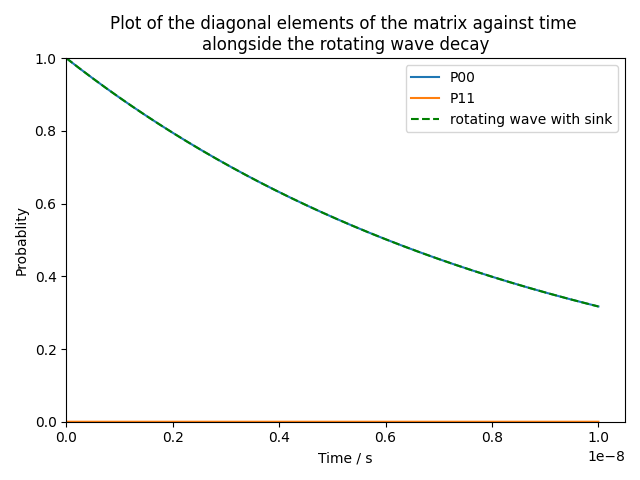
\includegraphics[width = 0.9\linewidth]{Figures/Redfield/Plot of redfield solution long time sink.png}
        \caption{Complete solution with sink
        }\label{fig:redfield full solution with sink}
    \end{subfigure}
    \caption{Plot of the full solution of the Redfield
    equation. On short timescales
    (\cref{fig:redfield full solution short timescales})
    the solution is seen to
    oscillate with a characteristic
    frequency of \(2.1\times{}10^{-13}\)s however
    at long timescales
    (\cref{fig:redfield full solution long timescales})
    the solution decays at the same rate as the
    Lindblad equation. The solution is
    also well behaved with the inclusion of
    a sink at the HCP site
    (\cref{fig:redfield full solution with sink}).
    }\label{fig:redfield full solution}
\end{figure}
In theory we should also be able
to solve the redfield equation
for multiple hydrogen sites, however
the additional computational complexity
rules this out. It is however possible to
approximate the behaviour
seen in the many site model
by placing a sink at
the HCP site
(\cref{fig:redfield full solution with sink}).
In this case
we again see good
agreement with the
lindblad equation.


